\documentclass[11pt,fleqn]{exam}

\setlength {\topmargin} {-.15in}
\setlength {\textheight} {8.6in}
\usepackage{enumerate}
\usepackage{amsmath}
\usepackage{amssymb}
\usepackage{xcolor}
\usepackage[colorlinks = true,
            linkcolor = blue,
            urlcolor  = blue,
            citecolor = blue,
            anchorcolor = blue]{hyperref}
\usepackage{listings}
\usepackage{color} %red, green, blue, yellow, cyan, magenta, black, white
\usepackage{graphicx}
\definecolor{mygreen}{RGB}{28,172,0} % color values Red, Green, Blue
\definecolor{mylilas}{RGB}{170,55,241}
\newcommand{\nn}{~\newline \noindent }
\newcommand{\mname}[1]{\mbox{\sf #1}}
\usepackage{float}


\begin{document}

\lstset{language=Matlab,%
    %basicstyle=\color{red},
    breaklines=true,%
    morekeywords={matlab2tikz},
    keywordstyle=\color{blue},%
    morekeywords=[2]{1}, keywordstyle=[2]{\color{black}},
    identifierstyle=\color{black},%
    stringstyle=\color{mylilas},
    commentstyle=\color{mygreen},%
    showstringspaces=false,%without this there will be a symbol in the places where there is a space
    numbers=none,%
    numberstyle={\tiny \color{black}},% size of the numbers
    numbersep=9pt, % this defines how far the numbers are from the text
    emph=[1]{for,end,break},emphstyle=[1]\color{red}, %some words to emphasise
    %emph=[2]{word1,word2}, emphstyle=[2]{style},    
}
	
\begin{center}
	{\large \textbf{COMPSCI 4X03}}\\[2mm]
	{\huge \textbf{Assignment 2}}\\[6mm]
	{\large \textbf{Mingzhe Wang}}\\[2mm]
	{\large \textbf{McMaster University}}\\[6mm]
	{\large \today}
		
\end{center}
	
\medskip
		
\subsection*{Problems 1}
\subsubsection*{without pivoting}
\begin{figure}[H]
  	\centering
  	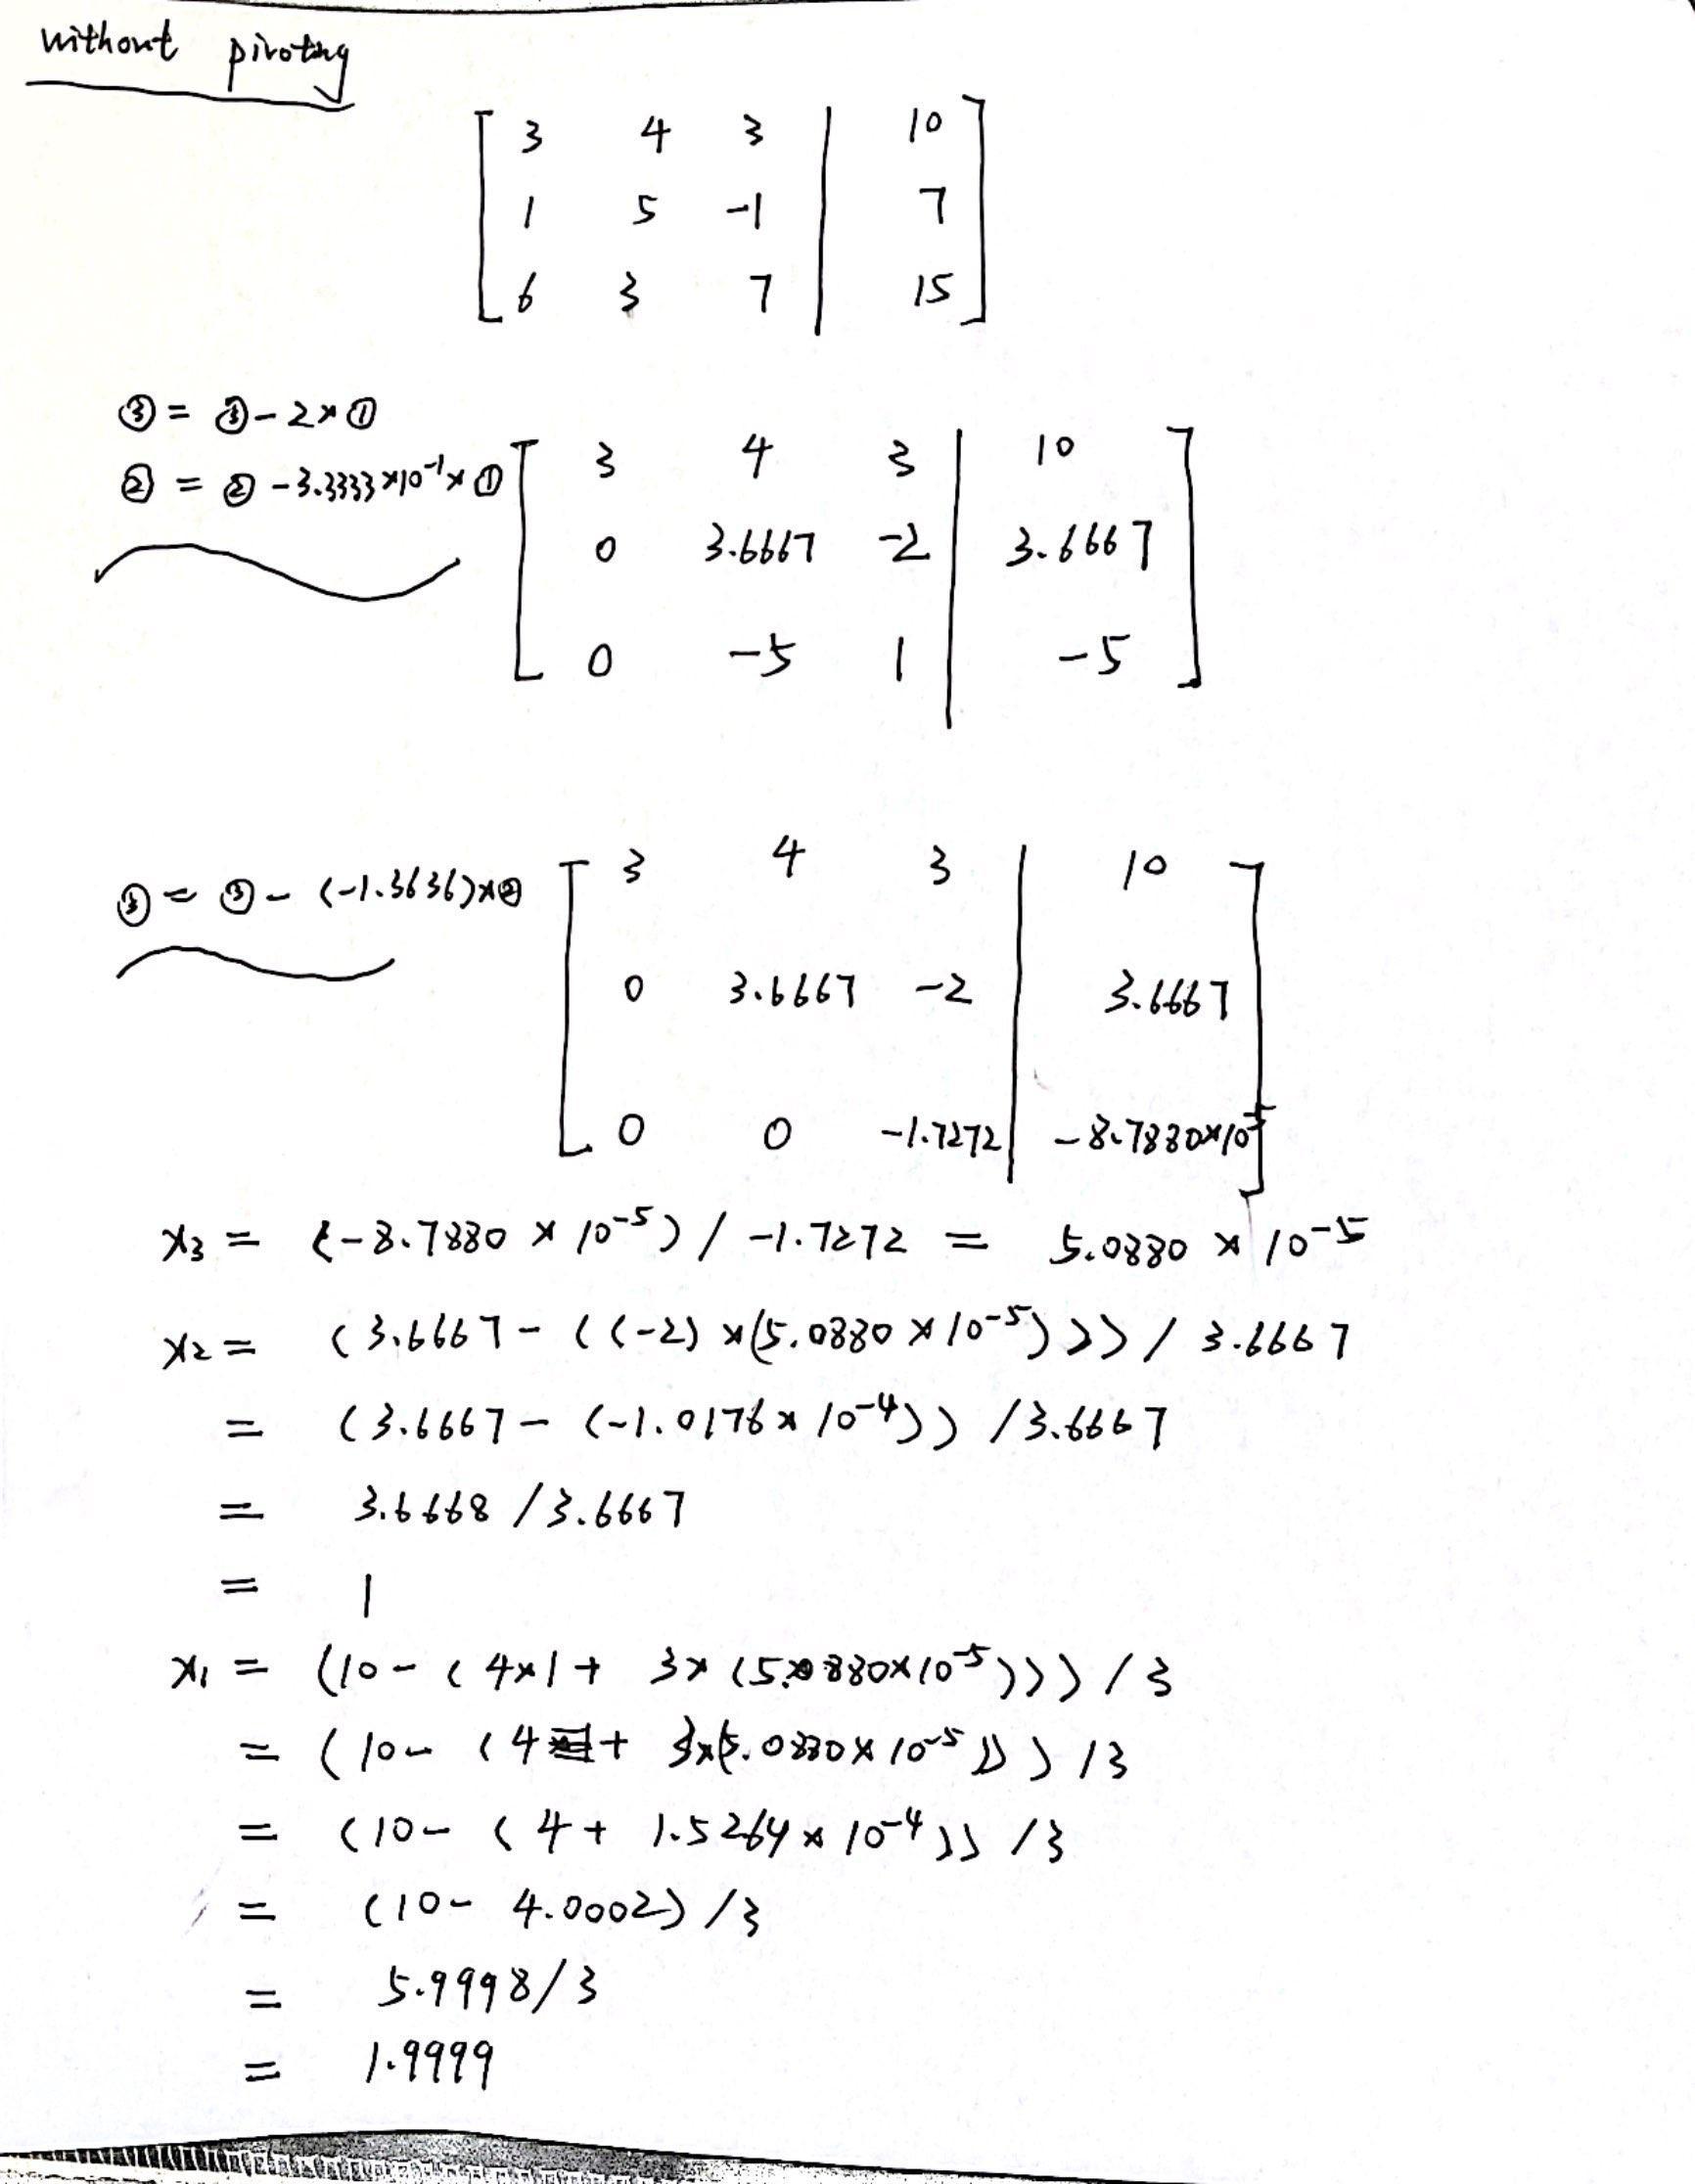
\includegraphics[width=0.6\textwidth]{q1_a}
\end{figure}
\subsubsection*{with partial pivoting}
\begin{figure}[H]
  	\centering
  	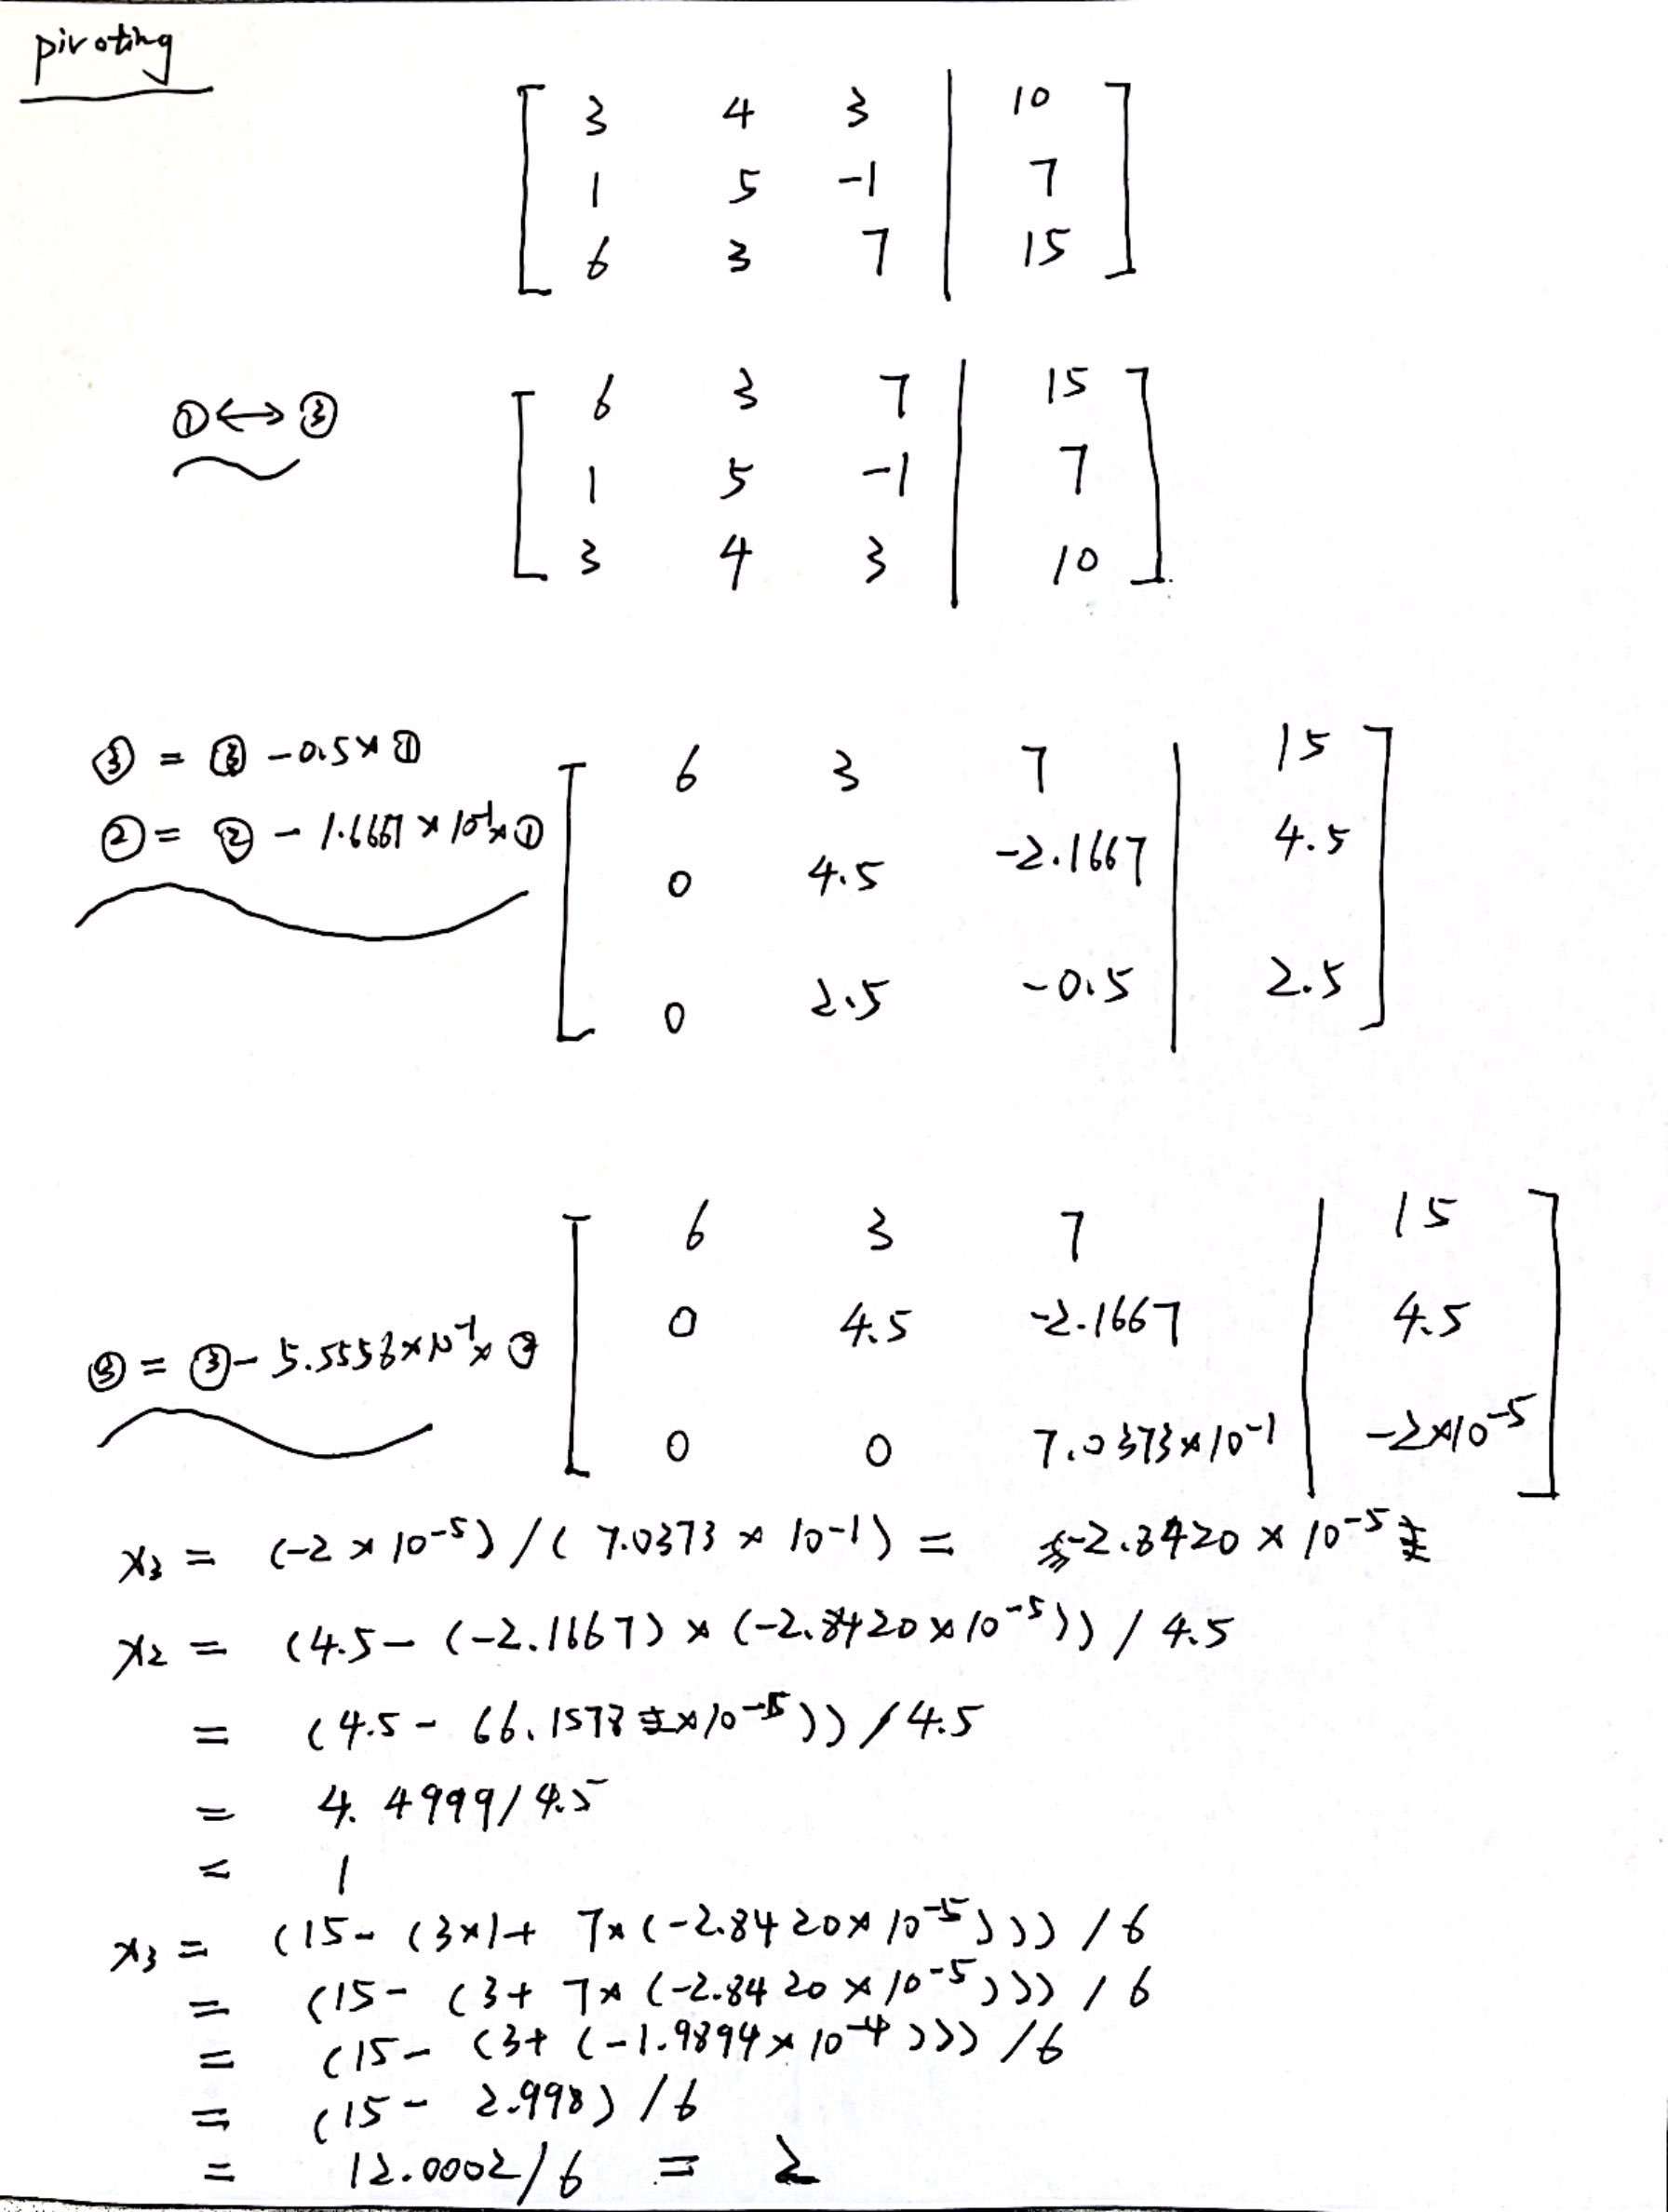
\includegraphics[width=0.6\textwidth]{q1_b}
\end{figure}

\subsection*{Problems 2}
\subsubsection*{values of $\epsilon$}
\begin{figure}[H]
  	\centering
  	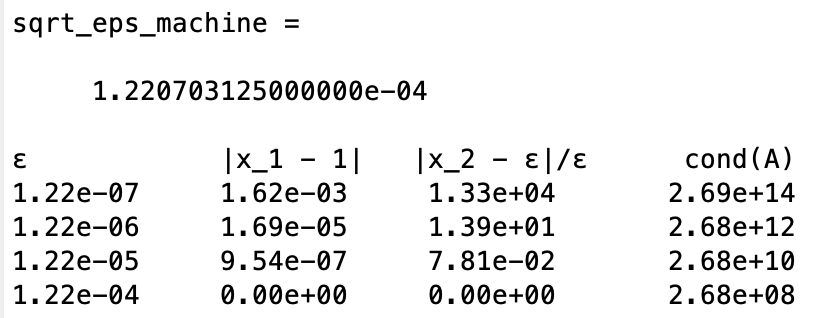
\includegraphics[width=0.6\textwidth]{q2}
\end{figure}
\subsubsection*{conclusion}
If $cond(A) \approx 10^k$, then about $k$ decimal
digits are lost when solving Ax = b. In this case, because matlab's default precision is 16 digits, when $cond(A) \approx 10^k$ and $\epsilon \approx 10^m$, then the relative error for $x_1 \approx 10^{k - 16}$ and the relative error for $x_2 \approx 10^{k - 16 - m}$.

\subsection*{Problems 3}
\subsubsection*{a}
\textbf{GE}
\lstinputlisting{GE.m}

~\newline
\textbf{GEPP}
\lstinputlisting{GEPP.m}

~\newline
\textbf{backward}
\lstinputlisting{backward.m}

\subsubsection*{b}
\lstinputlisting{main_ge.m}

\subsubsection*{c}
\begin{figure}[hbt!]
  	\centering
  	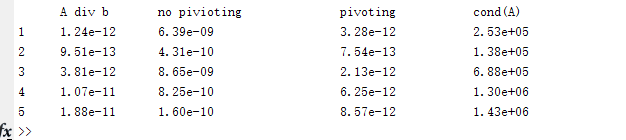
\includegraphics[width=1.0\textwidth]{q3_c}
\end{figure}

\subsubsection*{d}
As the condition numbers get larger, relative errors of all three methods get larger. If the condition number $\approx 10^m$ and the relative error $\approx 10^k$, then they have a relation $k - m = 16$, where 16 is matlab's default precision digit number. In other word, If $cond(A) \approx 10^k$, then about $k$ decimal digits are lost when solving Ax = b. 

\newpage
\subsection*{Problems 4}
\begin{figure}[hbt!]
  	\centering
  	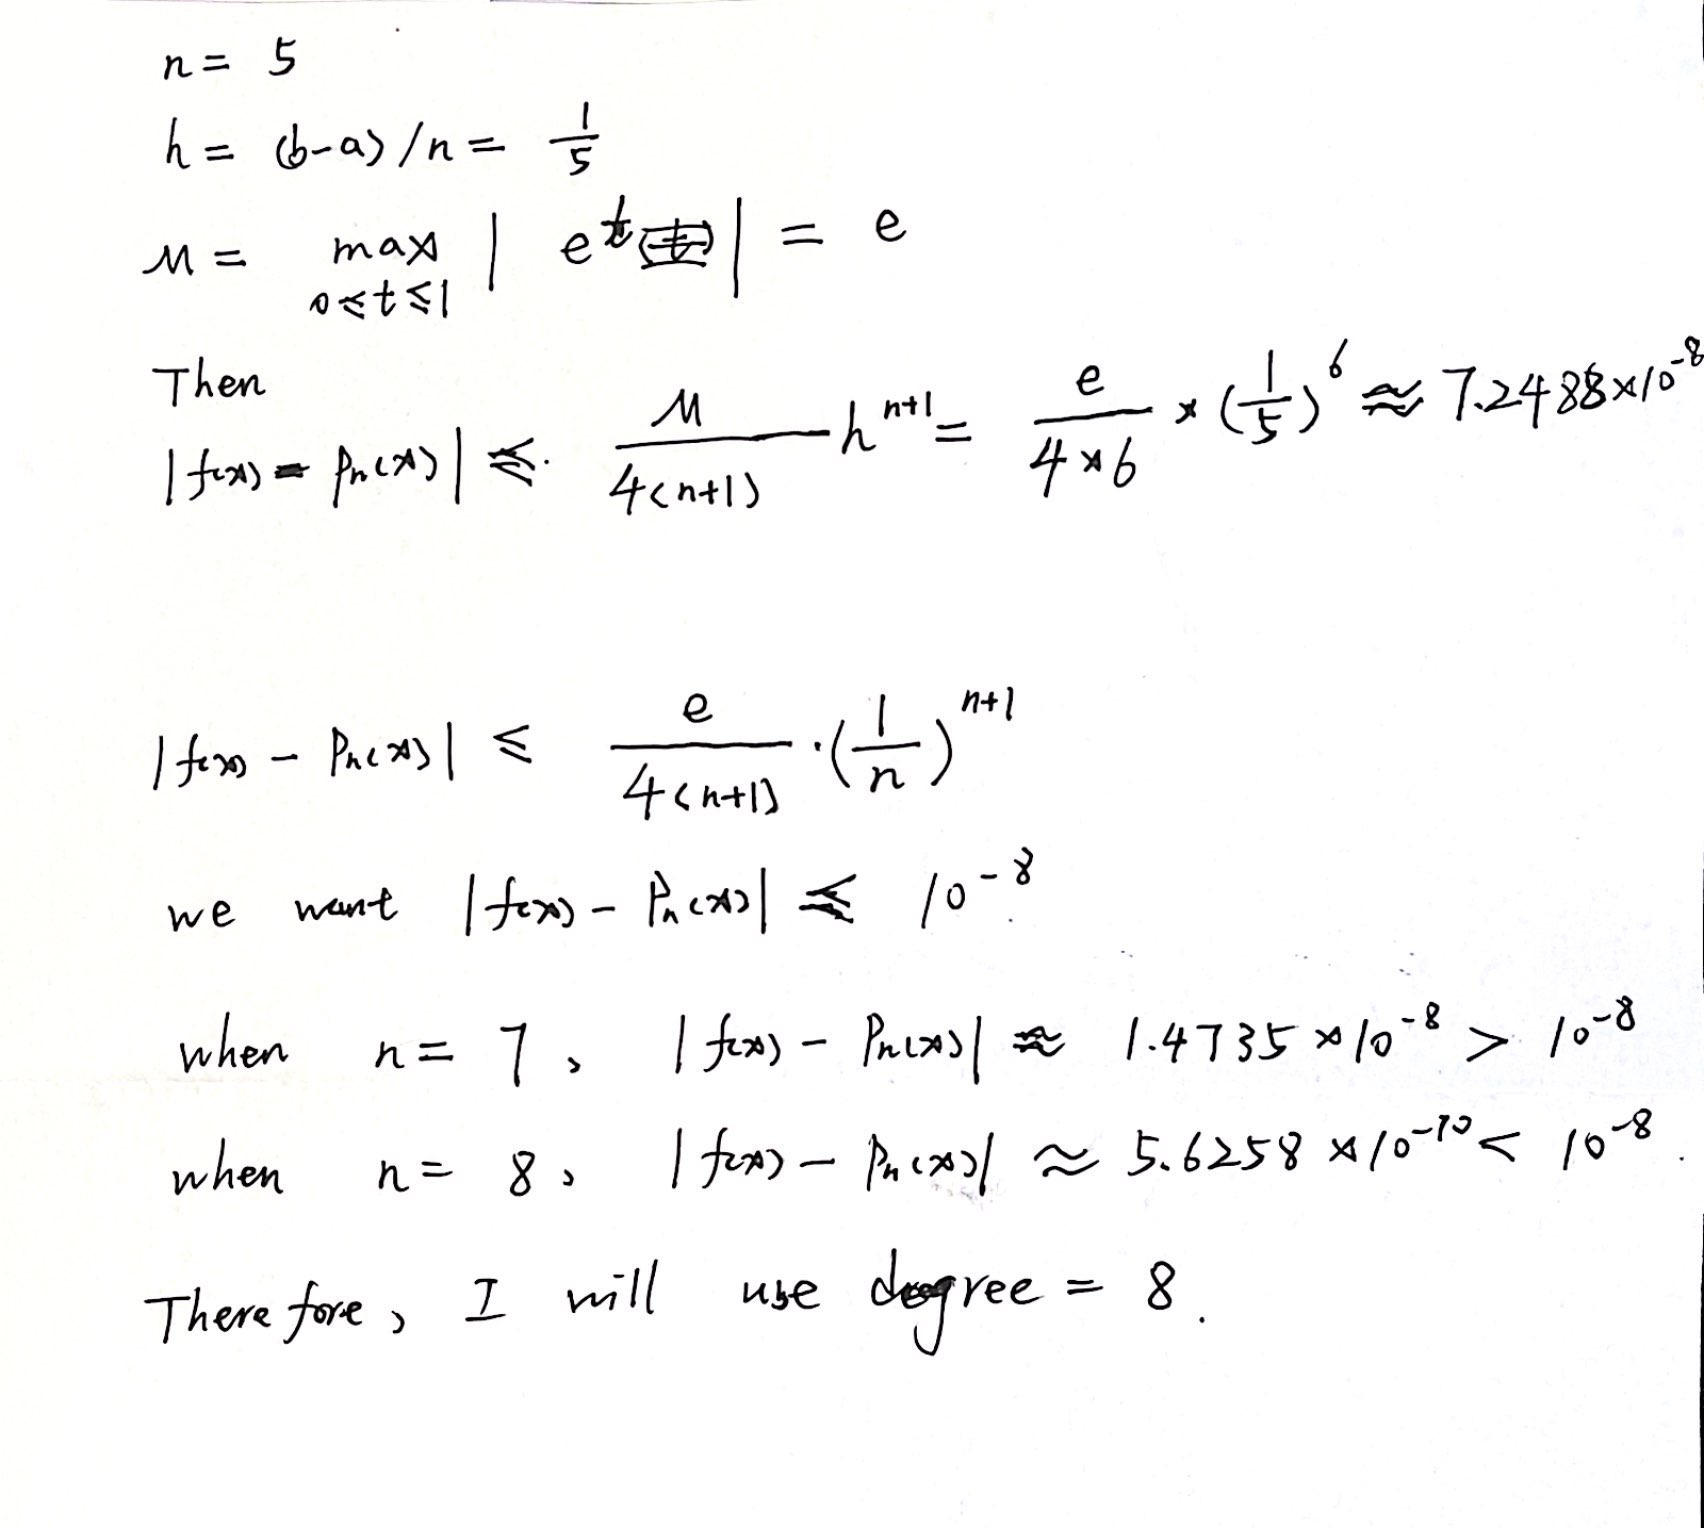
\includegraphics[width=0.8\textwidth]{q4}
\end{figure}

\subsection*{Problems 5}
\lstinputlisting{q5.m}

\subsubsection*{a}
The approximation for $\sqrt{0.05+1}$ is $1.024692660787484e+00$.
The approximation for $\sqrt{0.15+1}$ is $1.072381890220326e+00$.

\subsubsection*{b}
\begin{figure}[hbt!]
  	\centering
  	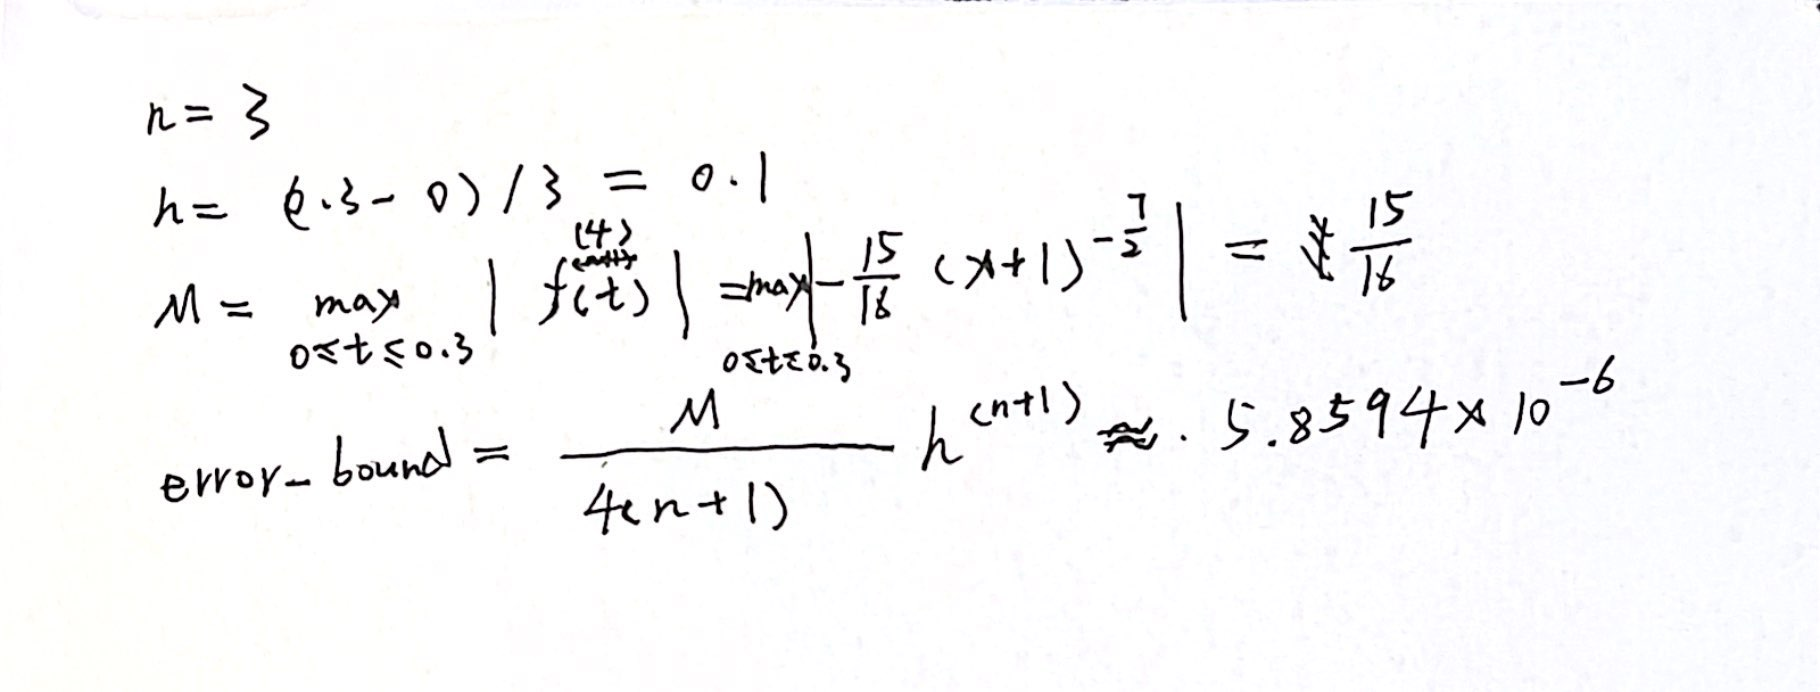
\includegraphics[width=0.8\textwidth]{q5_b}
\end{figure}

\subsubsection*{c}
As we can see from the figure, the error bound is always larger than the actual error.
\begin{figure}[H]
  	\centering
  	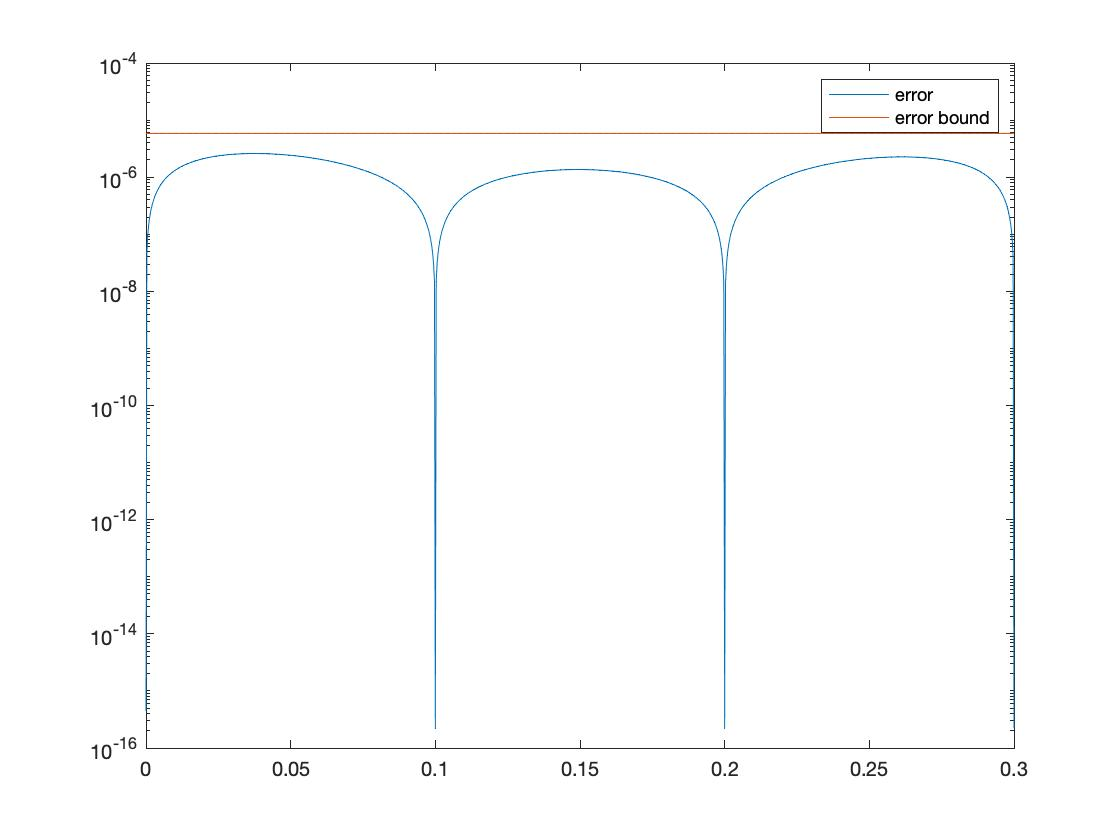
\includegraphics[width=0.6\textwidth]{q5_c}
\end{figure}

\newpage
\subsection*{Problems 6}
Below are four figures for $f(x) = |x|$ on $[-1,1]$.
\begin{figure}[H]
  	\centering
  	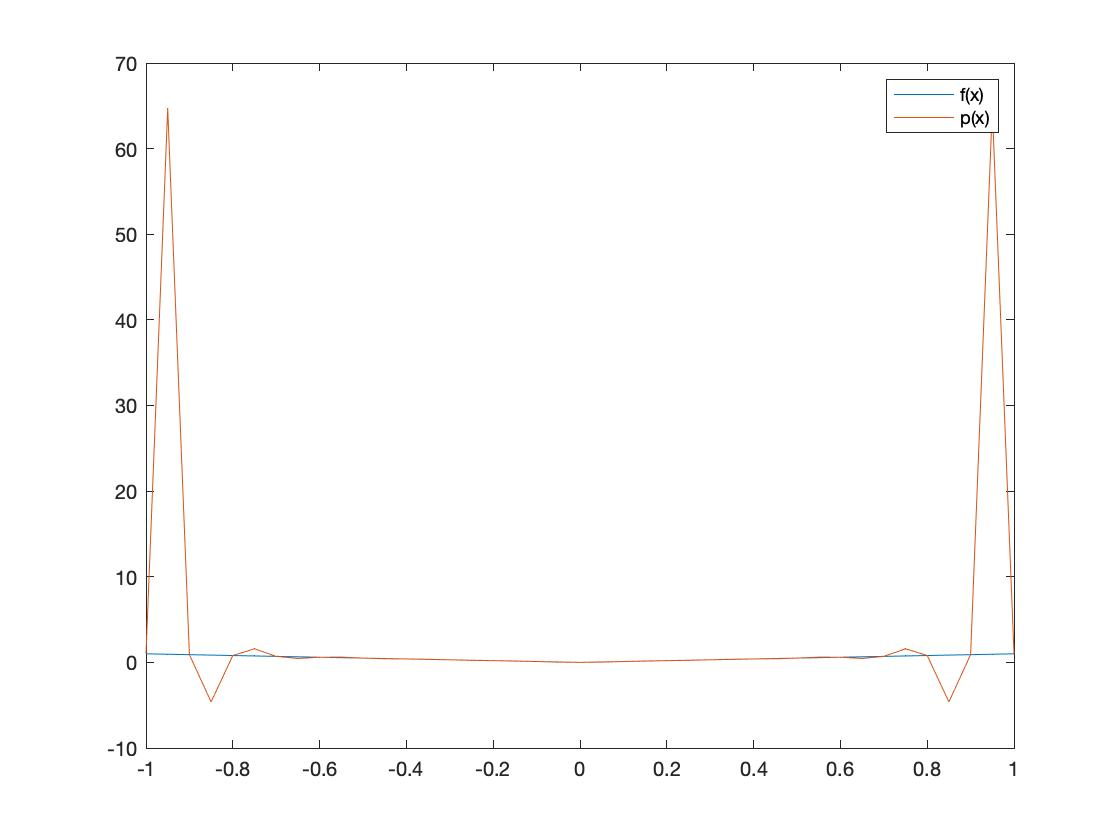
\includegraphics[width=0.7\textwidth]{q6_a}
  	\caption{$f(x)$ and $p(x)$ for equally spaced points}
\end{figure}

\begin{figure}[H]
  	\centering
  	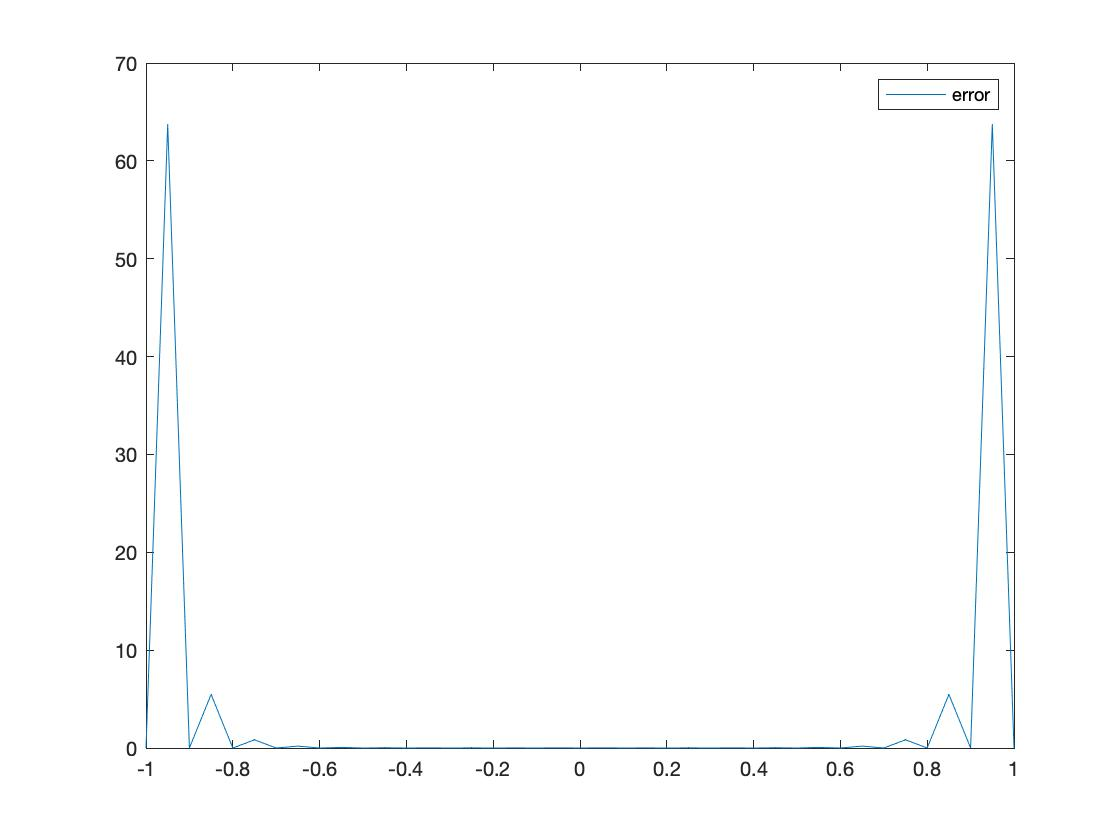
\includegraphics[width=0.7\textwidth]{q6_b}
  	\caption{error $|f(x) - p(x)|$ for equally spaced points}
\end{figure}

\begin{figure}[H]
  	\centering
  	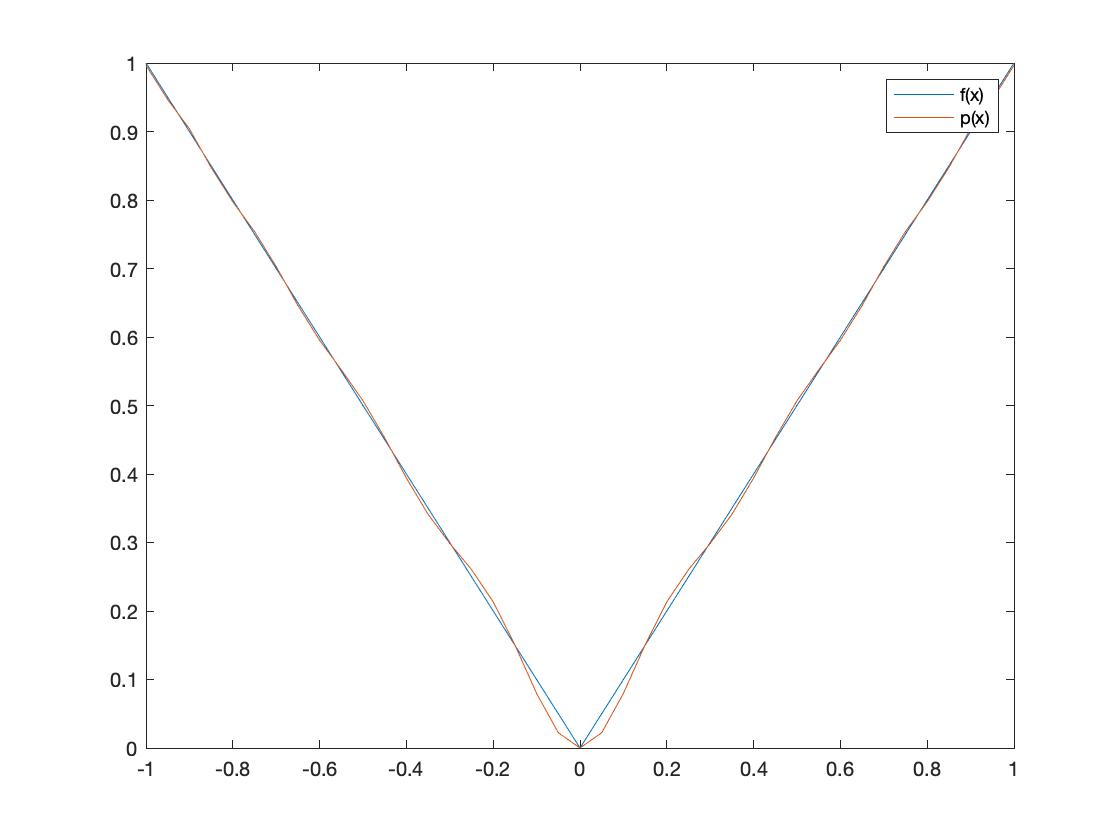
\includegraphics[width=0.7\textwidth]{q6_c_1}
  	\caption{$f(x)$ and $p(x)$ for Chebyshev points}
\end{figure}

\begin{figure}[H]
  	\centering
  	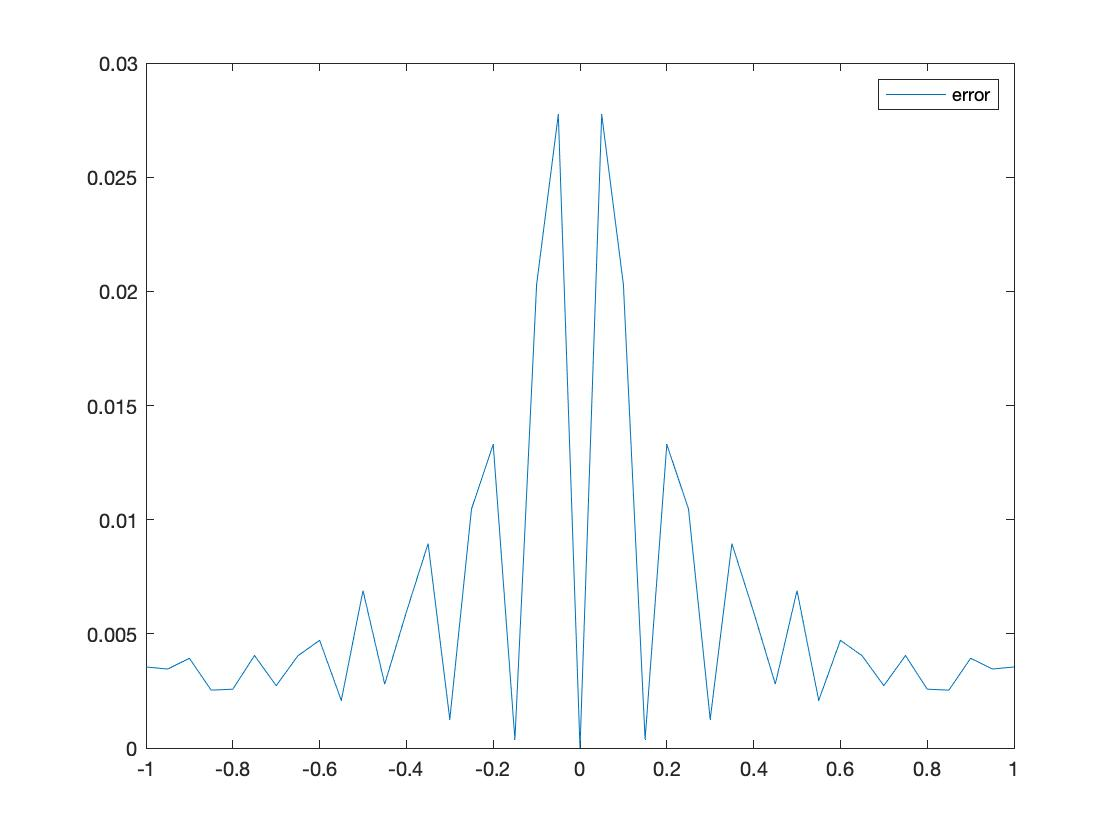
\includegraphics[width=0.7\textwidth]{q6_c_2}
  	\caption{error $|f(x) - p(x)|$ for Chebyshev points}
\end{figure}

\newpage
\subsection*{Problems 7}
Below are four figures for $f(x) = sin(x)$ on $[-\pi,\pi]$.
\begin{figure}[H]
  	\centering
  	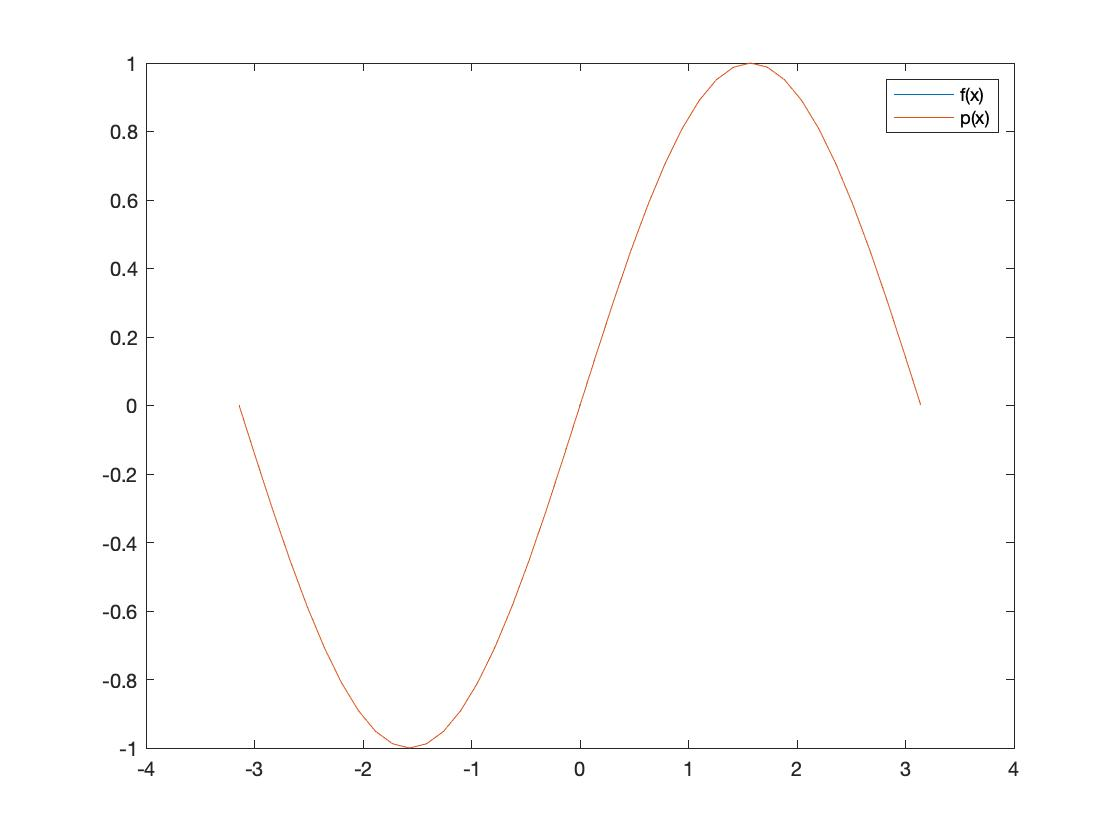
\includegraphics[width=0.7\textwidth]{q7_a}
  	\caption{$f(x)$ and $p(x)$ for equally spaced points}
\end{figure}

\begin{figure}[H]
  	\centering
  	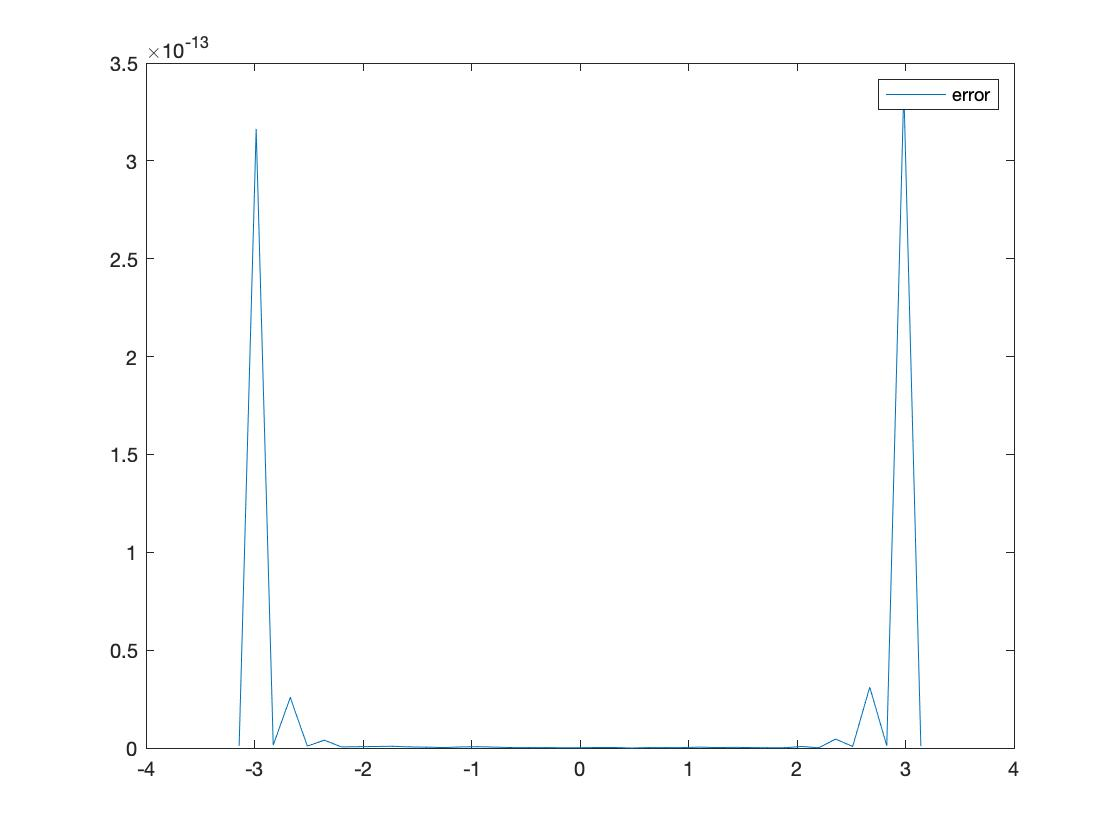
\includegraphics[width=0.7\textwidth]{q7_b}
  	\caption{error $|f(x) - p(x)|$ for equally spaced points}
\end{figure}

\begin{figure}[H]
  	\centering
  	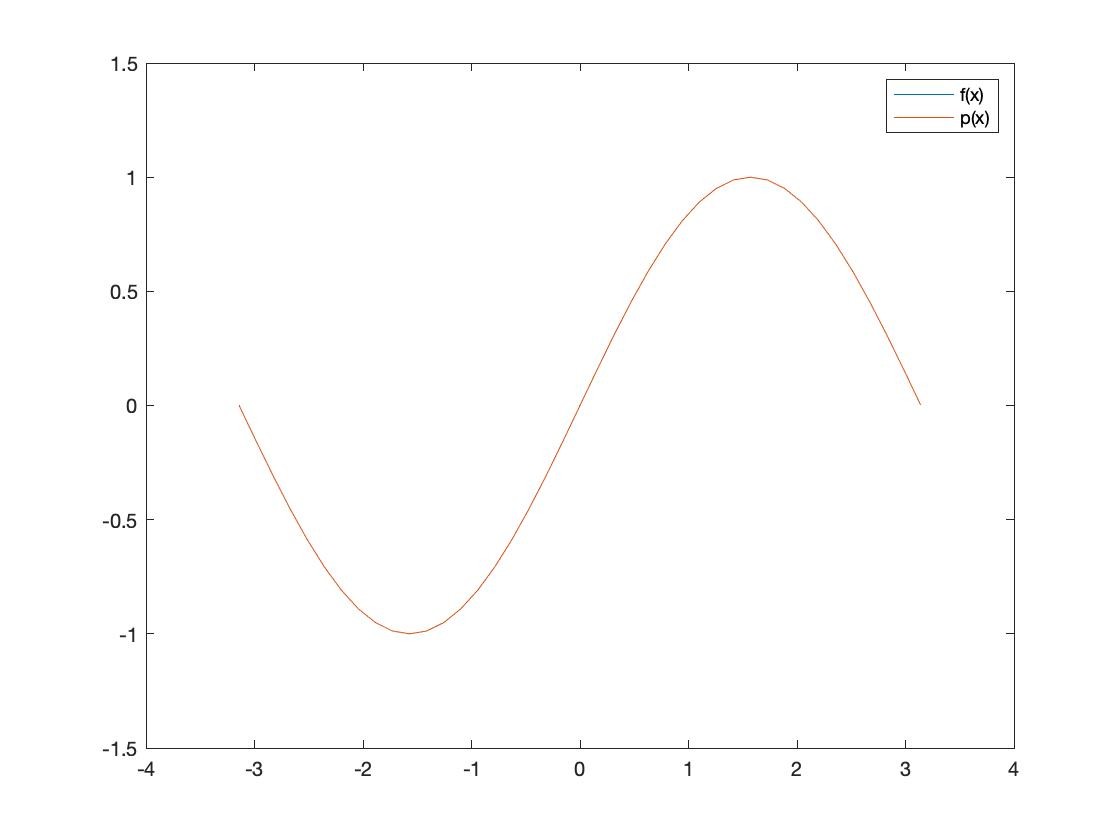
\includegraphics[width=0.7\textwidth]{q7_c_1}
  	\caption{$f(x)$ and $p(x)$ for Chebyshev points}
\end{figure}

\begin{figure}[H]
  	\centering
  	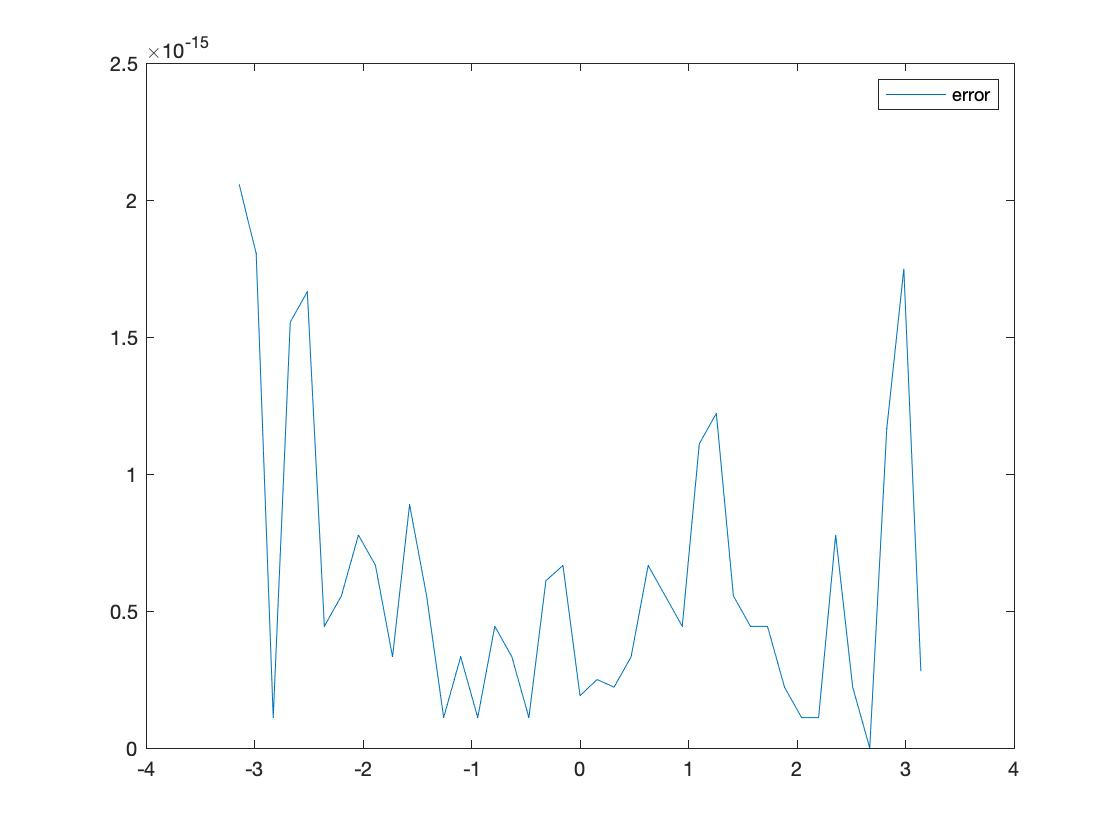
\includegraphics[width=0.7\textwidth]{q7_c_2}
  	\caption{error $|f(x) - p(x)|$ for Chebyshev points}
\end{figure}

\subsubsection*{explanation}
Compared between the equally spaced points and Chebyshev points, either for $f(x) = sin(x)$ or $f(x) = |x|$, interpolation on Chebyshev points has a lower error bound, which is because of Chebyshev points's Min-max property.\\
Compared between $f(x) = sin(x)$ and $f(x) = |x|$, either for the equally spaced points or Chebyshev points, $f(x) = sin(x)$ can be easily interpolated, because of its cyclicity.

\subsection*{Problems 8}
\textbf{newton}
\lstinputlisting{newton.m}

~\newline
\textbf{hornerN}
\lstinputlisting{hornerN.m}

\end{document}


